\documentclass[11pt]{article}

\usepackage[left=2cm, right=2cm, top=2cm]{geometry}
\usepackage[dvipdfmx]{graphicx}
\usepackage{float}
\usepackage{hyperref}

\hypersetup{
    colorlinks=true,
    linkcolor=black,
    filecolor=magenta,      
    urlcolor=blue,
}

\providecommand{\e}[1]{\ensuremath{\times 10^{#1}}}

\title{Project 2: Text Scroller}
\author{Jacob Boline}

\begin{document}
\maketitle

\section{Introduction}
In this project I was tasked with creating a design that would scroll text across the 8 digit, 7 segment display. It was required that on power-on the device must load a default message to display and begin scrolling it across the display. In addition, the display must have a mode where the user can program all 8 digits using the 16 switches that were on board. Finally, the device was required to utilize a Block-RAM module for storing the data.  To accomplish this project Vivado 2017.2 was used to simulate, synthesize, and implement System Verilog code for a Basys 4 DDR development board. The design files for this project can be found at \url{https://github.com/txjacob/SoC_FPGA}

\section{Experimental Plan}
\begin{figure}[H]
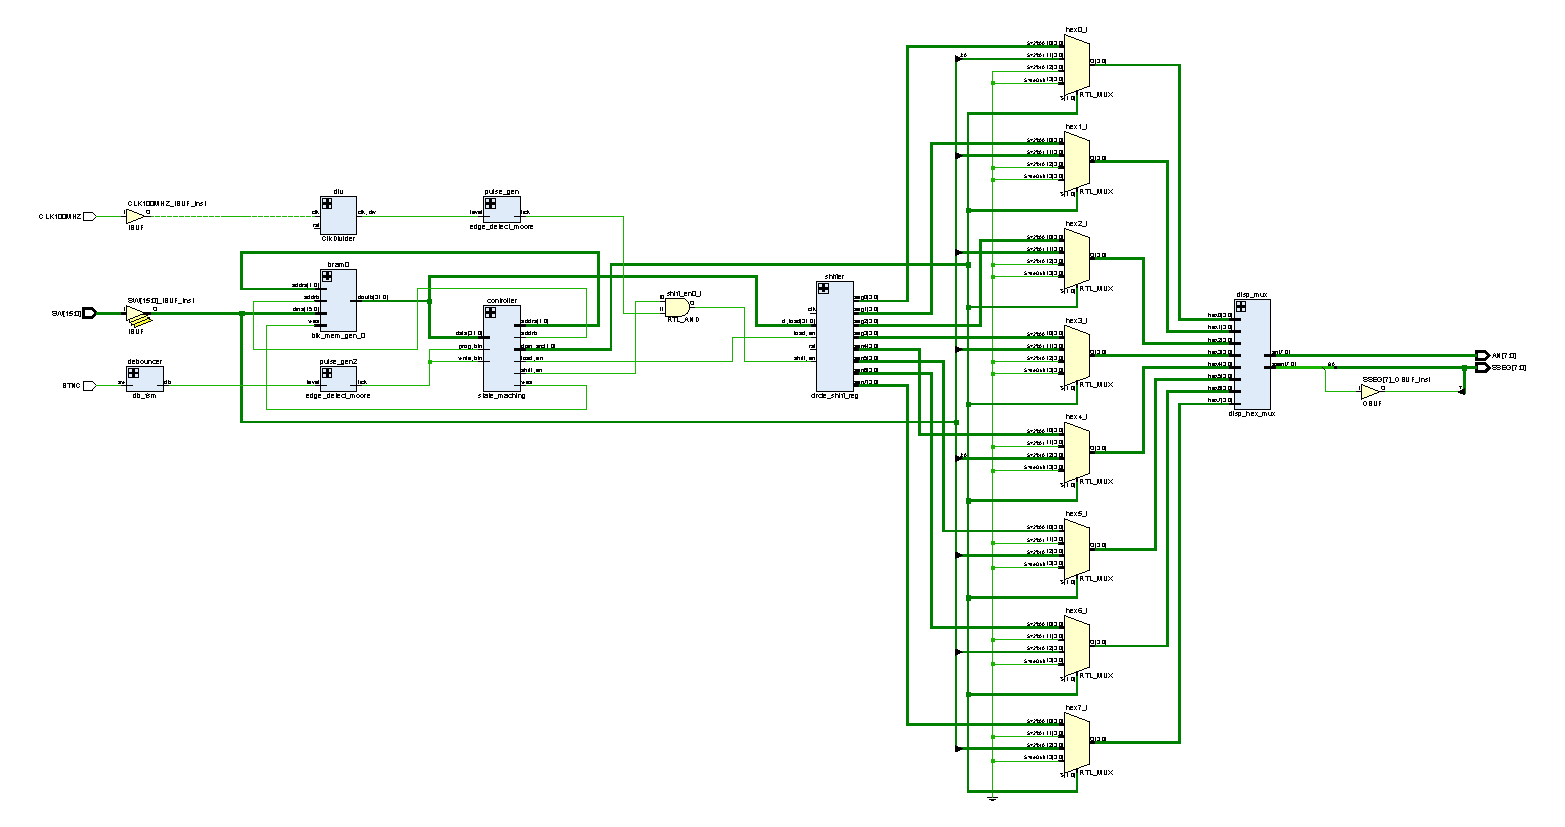
\includegraphics[trim={0.35cm 6.5cm 11cm 2.75cm}, clip,width=7 in]{./figures/schematic.eps}
	\centering
	\caption{Simplified block diagram of the input and control logic.}
	\label{fig:input_logic}
\end{figure}

Figure \ref{fig:input_logic} shows the input and control logic for the system. The most important module is the controller which is comprised of a state machine that has 8 states: init, load, run, prog0, prog1, inter0, inter1, and load\_reg. A diagram for this state machine can be seen in Figure \ref{fig:state_diagram}. 

\begin{figure}[H]
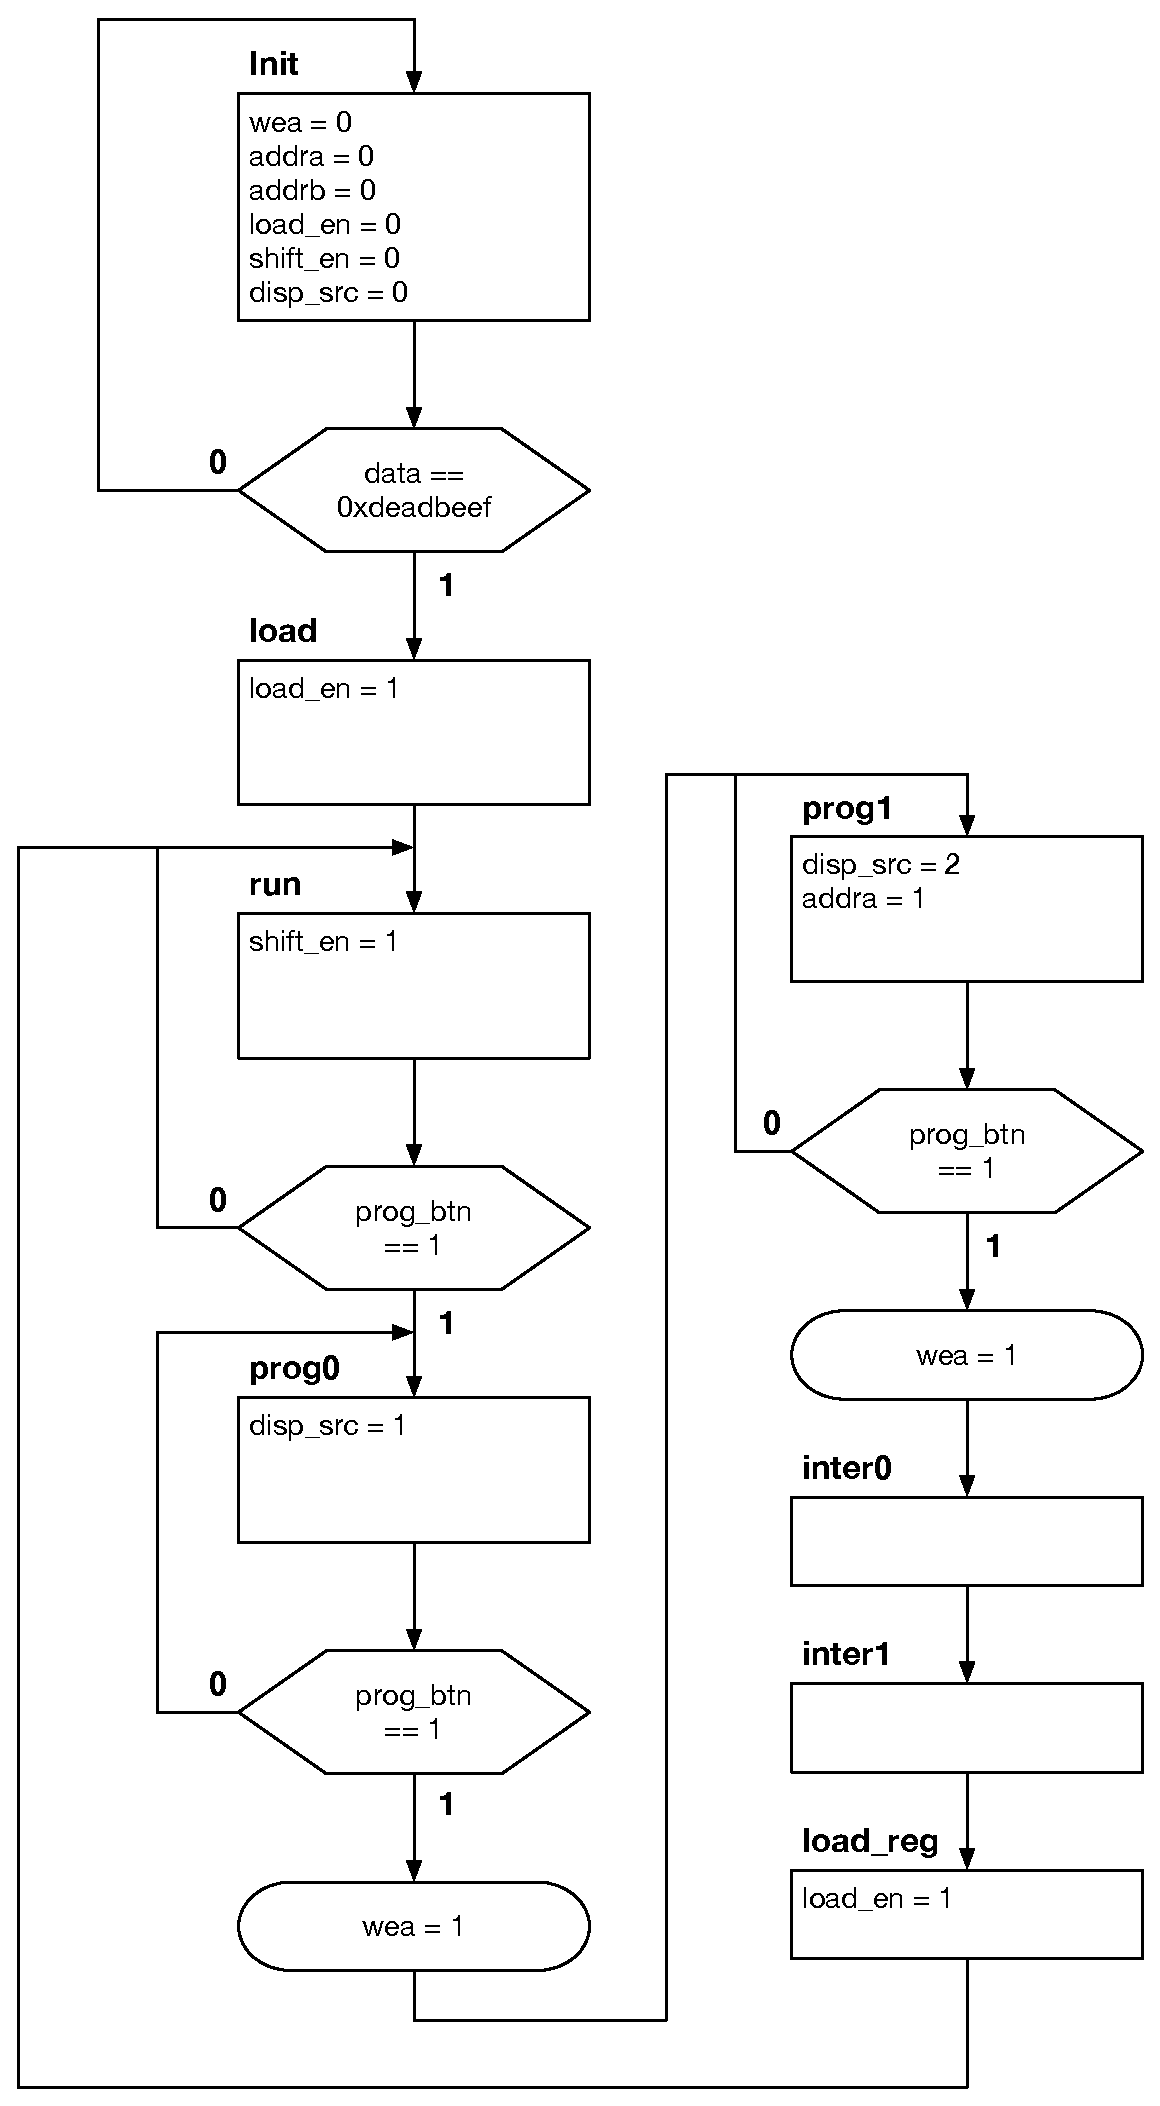
\includegraphics[width=4.5 in]{./figures/state_diagram}
	\centering
	\caption{State diagram for controller.}
	\label{fig:state_diagram}
\end{figure}

When the FPGA is first programmed the state machine will sit in the init state until the BRAM has properly initialized. Once this has occurred the state machine will load the shift register and move onto the run phase. The programming mode is controlled with the use of a single button. To achieve this functionality I fed the button through a debouncer and into a rising edge detector. This allows a short pulse to be generated when the button is pushed thus only triggering one action from the state machine. When the button is first pushed the programming mode is entered and the bottom 4 digits can be programmed. Once the button is pushed the data from the switches is latched into address 0 of the BRAM, and the top 4 digits can then be programmed. Pushing the button again causes the data from the switches to be latched into address 1 of the BRAM. After the programming state is left, the state machine goes through two delay states. The purpose of these states is to compensate for the 2 cycle latency of the data being programmed into the BRAM. Without them the shift register will try to load the data before it is ready.

The shift register features parallel loading, and shifts data in 4-bit chunks. This was created by building each 4-bit register individually than wiring them up to create an 8 element deep shift register. When wiring up the shift register I realized there would be a noticeable delay if I used the divided clock to load and shift the register. In order to overcome this I instead ran the shift register off of the main 100 MHz clock, and fed the divided clock through an edge detector and into the shift enable pin. Since the clock divider module will always be running I fed the shift\_en bit from the state machine through an AND gate with the clock divider to allow the shifting to be completely disabled.

\end{document}